
%%
% bayesian data analyses

% guessing parameter only used in language tasks, not in prior elicitation
% expt1a
%	- prevalence for categories (e..g "lions" that "have manes"):  
%         -  Beta(gamma, delta)  --- gamma (uniform 0 1); delta  (uniform 0 50)
% 		- using posterior on gamma for model
%   - prevalence prior for properties (e.g. "have manes"): 
%		- theta_across (uniform 0 1)	
%         -  Beta(gamma_within, delta_within)  --- gamma (uniform 0 1); delta  (uniform 0 50)
% 		-  using posterior on beta for model
% expt1b
%   - speaker optimality
%	- phi
% expt 2a
%  - Beta_across (gamma_across, delta_across) - 
%  - Beta_within (gamma_within, delta_within) -
%  - phi
% expt 2b
%   - speaker optimality (truth conditions)
%   - speaker optimality (implied prevalence)
%	- 2 phis (1 per task)





% mh 7/19
% in experiment 1 and model, take the speaker perspective when talking about how the model works

%todo after cogsci:
%-run additional contexts. e.g. separate dangerous and distinct.
%-look again at finer-grained truth judgement task?
%-think about the weird cases of generics in the literature. e.g. ``robins lay eggs''.
% - try an S2 model of prevalence judgement task, too. does it reduce to the L1 model?

% comments from workshop class 4/29
%
% why spend a lot of time in replication?
% 7 --- summary sentence 2nd paragraph to intro
% abstract worrisome
% look at study discussions -- move stuff to intro
%
% Lay eggs vs. Are female /// John is tall vs. ESB is tall [move even earlier]
% Move "a natural foil" earlier
%
% Maybe add talk of stereotypes?
% Craig: Use speaker / listener actors more; think about the person and the thing they're doing
% %
%  beef up penultimate paragraph in intro: talk about why distinctive and dangerous are important
% ---- unpack distinctive and dangerous (use experimental materials)
%
% TABLE for materials and experiment. 
% maybe set up replication-idea early.  and then go on.




% details
%
% Section 4: exp 2 intro
%% oceans underneath each sentence
%% connect back with behavior--- asymmetry, truth cond
%
% pre Exp 3: use 
% "endemic to the entire category"
% exp3a: jargon word 
% (reuse penultimate intro paragraph throughout) [maybe make higher level version of this paragraph for intro]
%
% pre-experiments, "Like Exp 2c, 3b did BLAH but differed "
%
% add more to figure captions?
%
%
% seeds of very last paragraph in earlier
%
% in conclusion: what do the tools allow us to do? (e.g. w/ stereotyping) 
% differences in prior knowledge --> how does this contribute to language change?
% 

\documentclass[10pt,letterpaper]{article}

\usepackage{setspace}
%\doublespacing
\usepackage{geometry}
\geometry{legalpaper, margin=1in}

\usepackage{pslatex}
\usepackage{apacite}
\usepackage{url}
\usepackage{graphicx}
\usepackage{caption}
\usepackage{subcaption}
\usepackage{listings}
\usepackage{color}
\usepackage{textcomp}
\usepackage{amsmath}
\usepackage{amssymb}
\usepackage{wrapfig}
\usepackage{lipsum}


\graphicspath{{figures/}}

\def\signed #1{{\leavevmode\unskip\nobreak\hfil\penalty50\hskip2em
  \hbox{}\nobreak\hfil(#1)%
  \parfillskip=0pt \finalhyphendemerits=0 \endgraf}}

\newsavebox\mybox
\newenvironment{aquote}[1]
  {\savebox\mybox{#1}\begin{quote}}
  {\signed{\usebox\mybox}\end{quote}}


 \newcommand{\denote}[1]{\mbox{ $[\![ #1 ]\!]$}}

\definecolor{Red}{RGB}{255,0,0}
\newcommand{\red}[1]{\textcolor{Red}{#1}}  
\definecolor{Green}{RGB}{10,200,100}
\newcommand{\ndg}[1]{\textcolor{Green}{[ndg: #1]}}  

\usepackage{titlesec}

\setcounter{secnumdepth}{4}

\titleformat{\paragraph}
{\normalfont\normalsize\bfseries}{\theparagraph}{1em}{}
\titlespacing*{\paragraph}
{0pt}{3.25ex plus 1ex minus .2ex}{1.5ex plus .2ex}



\title{Generic language is vague yet \{rationally / pragmatically\} \{used / understood\}}

\author{{\large \bf Michael Henry Tessler} (mtessler@stanford.edu)\\ {\large \bf Noah D. Goodman} (ngoodman@stanford.edu) \\
  Department of Psychology, Stanford University}
 
\begin{document}

\maketitle


\begin{abstract}
\ndg{to revise: higher level, less technical, more punchy.}
Generic utterances (e.g. ``Dogs bark.'') are the primary vessel by which speakers express ideas about categories in the world and are ubiquitous in everyday conversation. 
Despite their prevalence, the meanings of generic statements are puzzling to formal theories. 
It is believed that generic utterances behave somewhat like quantified ones (e.g. ``Most dogs bark.''). 
If this is correct, however, there should be some threshold on the percentage of the category that must display the property (e.g. some criterion number of dogs that bark) for the utterance to be true.
This threshold is notoriously difficult to define for generics, which are flexible enough to be true based on very little evidence while also implying near-universality of the property. 
Here, we formalize a semantics and pragmatics for generic language understanding, based on the idea that generics are vague: The threshold for acceptance is represented as an unknown property of the language and is actively reasoned about in context by a listener who assumes she is in conversation with an informative speaker. 
We explain how this simple semantics can account for two central phenomena surrounding generic language: The flexible conditions by which a generic is true and the variable implications of generic language. 
Inferences from the model are driven largely by the listeners' \emph{a priori} beliefs about the property, which we measure empirically.
This demonstrates that the semantics of generic statements can treated as scalar and suggests that listeners' expectations in the form of prior beliefs heavily govern generic interpretation. 


\textbf{Keywords:} 
generics; semantics; probabilisitic pragmatics
\end{abstract}

Imagine talking with a 2-year-old about colors.
Colors are difficult to describe because they take shape in different physical forms and the function of color is abstract.
You might offer the toddler something generic like, ``Apples are red.''. 
Few would argue with the truth of this sentence, yet its precise meaning is difficult to specify. 

This type of utterance is generic \cite{Carlson1977, Leslie2008} in that it conveys a generalization about a category (e.g. \emph{apples}).  
Generics are one of the simplest linguistic constructs and are ubiquitous in everyday conversation, child-directed speech \cite{Gelman2008}, and are the primary vessel by which speakers discuss social categories, making them central to communicating stereotypes \cite{GelmanEtAl2004, Cimpian2010motivation, Leslie2015}.
They have no explicitly marked operator and yet children as young as two or three correctly understand that they refer to categories and not just a plurality in a scene \cite{Cimpian2008}. 
They are believed to be essential to the growth of conceptual knowledge \cite{Gelman2004} and how we represent kinds \cite{Leslie2008}.
Despite their centrality to cognitive development and everyday conversation, a formal account of generic meaning remains elusive.

At first glance, generics seem like universally-quantified statements (i.e. ``All apples are red.''), but unlike universals, generics are resilient to counter-examples like \emph{Granny Smith apples}. 
Interpreting the generic as meaning ``most'' (i.e. ``Most apples are red.'') captures many cases, but cannot explain why ``Lions have manes'' and ``Mosquitos carry malaria.'' both seem true, despite the fact that among lions, only the adult males have manes and that a very small percentage of mosquitos actually carry malaria.
The only quantifier that could satisfy all of these conditions is the weak ``some'' (i.e. ``Some apples are red.'').  
Yet, the semantics for ``some'' is not the semantics of generics:  Generics have strong implications. 
Listeners are wont to interpret the sentence as applying to \emph{nearly all} of a category \cite{Gelman2002, Cimpian2010}. 
``Some apples are red.'' does not carry the same generalizability as ``Apples are red.''.
Additionally puzzling is the fact that while ``Lions have manes.'' is a fine generic utterance, ``Lions are male.'' is not, even though the prevalences of the two properties are the same for the category of lions.

%The semantics of generics is often contrasted with that of quantifier sentences, which are classically understood in terms of the prevalence of a property and are straightforward to evaluate for truth. 
%For example, ``\emph{Some} shoes have arch support.'' is true because there are shoes that do. 
%``\emph{Most} shoes have arch support.'' is probably true because probably more than half of shoes do have support. 
%``\emph{All} shoes have arch support.'' is definitely not true because of the existence of Vibram 5 toes, flat sandals, and many others.
%But what about ``Shoes have arch support.''? 
%Is there some prevalence beyond which the generic becomes true?
%Prevalence based accounts of generic meaning are difficult to defend. 

\subsubsection{The semantics and pragmatics of generic language  (400 words to this point)}

What could be the stable meaning of a generic given this extreme flexibility? 
We propose these phenomena can be explained as the effects of pragmatic inference filling in a meaning that is underspecified in the language. 
Pragmatic reasoning in communication has recently been formalized in probabilisitic models of language understanding \cite{Frank2012, Goodman2013, Franke2009} and explain how assumptions of truthful and informative interlocutors \cite{Clark1996, Grice1975, Levinson2000} produce rich meanings of linguistic expressions in context. 
We build upon this tradition to explain the semantics and pragmatics of generic language: We posit that generics are a vague description of prevalence in much the same way that gradable adjectives like \emph{tall} are vague descriptions of height. 
To understand the vagueness of ``tall'', consider the criteria by which a person is ``tall'' (e.g. \emph{$\sim$ 6 feet}) versus the conditions for a building to qualify as ``tall'' (e.g. \emph{$\sim$ 1000 feet}).
This context-sensitivity of meaning can be accounted for by positing the semantics of the word (``tall'') is a distribution over criteria (``anything could count as tall given the right context''). 
Probabilistic pragmatic approaches have shown how this uncertainty is resolved by a listener consulting her beliefs about the domain in question (``what are probable heights of a person?'') as well as taking into account the communicative force of a speech act (``why did the speaker bother to say ``John is tall'' when he could have not said anything?'') \cite{Lassiter2013, Qing2014}.
We present a semantics of generics can be thought of in the same way, as a vague description of the prevalence of a property.
%listeners arrive at rich interpretations of utterances by considering the thought-processes of a speaker whose goal is to be informative.
%The has provided formal, computational accounts of understanding utterances with quantifiers \cite{Goodman2013}, gradable adjectives \cite{Lassiter2015}, and nonliteral usages \cite{Kao2014}.
% for by treating the condition for tallness (i.e. the threshold beyond which something counts as tall) as an unknown property of the language, and modeling the listener as inferring this threshold in context \cite{Lassiter2015}. 
%The fact that the distributions of heights for buildings and people are different, and that listeners expect speakers to be for vague adjectives.
%
%
%The meanings of words are often embedded in a conversational context.
%Language understanding is a special case of social cognition---interlocutors think about one another when producing and interpreting utterances.  
%
%Recently, the Rational Speech-Act theory has been extended to account for gradable adjectives like \emph{tall}, which lack single, context-invariant meanings. 
%
%
%We propose that generics are vague in the same way that gradable adjectives, like \emph{tall}, are vague. 

We propose the literal semantics of a generic sentence ``K has F'' (e.g. ``Lions have manes.'') is a standard truth-functional, threshold meaning such that a category in question K has property F if the prevalence $x$ of F within K is greater than some threshold $\theta_{generic}$.
%
\begin{flalign}
\denote{\text{K has F}} = \{x^{\text{F}}_{K} : x^{\text{F}}_{K} = p(\text{F} | \text{K}) > \theta_{generic}\} \label{eq:literalgeneric}
\end{flalign}
%
The threshold $\theta_{generic}$, however, is left underspecified in the semantics.
Listeners have uncertainty about the threshold $\theta_{generic}$ \emph{a priori} and actively must reason about it in context to derive a realistic but informative meaning. 

The probabilistic model for generic interpretation, with an uncertain prevalence threshold is specified by:
%
\begin{flalign}
& P_{L_{1}}(x , \theta \mid g) \propto P_{S_{1}}(g \mid x, \theta) \cdot P(x) \cdot P(\theta) \label{eq:L1}
\end{flalign}
%
Eq.~\ref{eq:L1} is a model of a listener ($L_{1}$) who has been told a generic statement $g$ (e.g. ``Lions have manes.''). She has uncertainty about the prevalence of the property $x$ (``how many lions have manes?'') as well as the meaning of the generic $\theta$ (``what does this sentence even mean?''), and is trying to figure out what these are. 
$P(\theta)$ represents the listener's \emph{a priori} beliefs about the semantic variable $\theta$; we assume no informative beliefs about the threshold (i.e. $\theta \sim \text{Uniform}(0,1)$).
The listener resolves her uncertainty, in context, by consulting her prior beliefs about the property $P(x)$ and assuming that utterance was produced by a speaker $S_{1}$, whose goal was to be informative about the prevalence of the property $x$:
%
\begin{flalign}
& P_{S_{1}}(g \mid x, \theta) \propto \exp(\lambda \ln {P_{L_{0}}(x \mid g, \theta)}) \label{eq:S1}
\end{flalign}
%
The speaker knows the prevalence $x$ (e.g. knows that adult, male lions have manes). 
The listener ($L_{1}$) believes the speaker ($S_{1}$) to actually know the threshold $\theta$, and be a soft-max optimally informative speaker to a degree governed by $\lambda$ \cite{Luce1959}. 
This intuitive theory of a speaker is used to resolve this threshold and the prevalence $x$ by assuming the speaker was trying to be informative to a hypothetical literal listener:
%
\begin{flalign}
& P_{L_{0}}(x \mid g, \theta) \propto {\delta_{\denote{g(\theta)}(x)} P(x)} \label{eq:L0}
\end{flalign}
%
This idealized listener ($L_0$) has access to the threshold $\theta$ and thus knows exactly what the speaker meant to communicate. 
The literal listener simply uses Bayes' Rule where the likelihood function $\denote{g(\theta)}: X \rightarrow \text{Boolean}$ is a truth-function specifying the literal meaning of the generic given a threshold $\theta$, as in Eq.~\ref{eq:literalgeneric}. 
%The literal content in Eq.~\ref{eq:L0} is given by $\denote{g(\theta)}= \{x | x > \theta \}$ as in Eq.~\ref{eq:birds}.

This is a ``lifted variable'' pragmatics model because $\theta$, traditionally thought to be part of the semantic content of the utterance (and thus perfectly transparent to all in the conversation), has been underspecified in the semantics but is locally resolved through pragmatic reasoning.
How does a listener arrive upon a threshold? 
\citeA{Lassiter2013} demonstrated the inference about the threshold is a balance between truthfulness and informativity. 
Consider again the example of ``John is tall''. 
To make ``tall'' maximally truthful, the listener would set $\theta$ to be very low (e.g. 2 feet tall); no matter what John's height actually is, the utterance will be true since the threshold for tallness is so low. Here, truthfulness would be maximized. 
 Truthfulness is not the only constraint in conversation however; there is also the pressure to be informative. 
 A maximally informative ``tall'' would correspond to a threshold that carries with it the maximum surprisal or information gain on the part of the listener. 
 This would be a threshold that very few individuals could cross (e.g. 7 feet tall); this would correspond to something like ``the tallest''. 
 The lifted-variable pragmatics model seeks a balance between these two pressures. 
 The result is a threshold that signifies that ``John is tall'' means he is ``significantly taller than average''.
 
Eq.~\ref{eq:L1} is a model of generic interpretation: Upon hearing a generic, what prevalence is a listener likely to infer?
A generic production rule would then naturally be specified by a speaker who has this sort of listener in mind:
%To explain the different conditions under which a generic utterance can be true, we extend the lifted-threshold model of \citeA{Lassiter2013} to include a model of a speaker who is deciding whether or not to produce the utterance. 
\begin{equation} 
P_{S_{2}}(g \mid x) \propto  \sum_{\theta} P_{L_{1}}(x , \theta \mid g) =  P_{L_{1}}(x \mid g)
\label{eq:S2}
\end{equation}
%
The speaker in \eqref{eq:S2} considers the thought-processes of the listener in Eq.~\eqref{eq:L1}, and decides if the generic $g$ is a good way to vaguely describe the prevalence $x$. 
This decision is with respect to one or more alternative speech-acts, which here we take to be the act of saying nothing\footnote{The results are equivalent both when the alternative is stipulated to be (1) the negation:  ````Lions have manes'' is false'' as well as (2) the generic of the negation i.e. ``Lions do not have manes''. These alternatives are analogous to alternatives to ``John is tall'' of ``John is not tall'' and ``John is short'' in the vague adjective case.}. 
Importantly, $S_{2}$ doesn't actually have access to the threshold $\theta$, but knows that $L_{1}$ is thinking about it, and marginalizes over possible inferred values. 
Eq.~\eqref{eq:S2} is a model of generic production: For a given prevalence, is the generic a good thing to say?

\subsubsection{Generics have flexible truth conditions (1400 words to this point)} 

We tested the degree to which Eq.~\eqref{eq:S2} predicted that a given category--prevalence pair (e.g. ``Lions'' and ``have manes'') would result in a good generic (e.g. ``Lions have manes.''). 
 The probabilisitic model is fully specified by Eqs.~\eqref{eq:literalgeneric} -- \eqref{eq:S2}, with the exception of the speaker rationality parameter $\lambda$ and the prior distribution on prevalences $P(x)$. 
 We use Bayesian data analytic techniques to integrate out $\lambda$, which is not of theoretical interest here. 
 $P(x)$ describes the belief distribution on the prevalence of a given property (e.g. ``have manes''). 
 This distribution is conceivably different for different types of properties. 
 Thus, we measure it empirically by asking participants ($n=30$) about the prevalence of different types of properties for many different animal categories\footnote{Our experiments stay within the animal kingdom because we expect there to be considerably less variability in participants beliefs about animals than about other types of categories (e.g. social categories)}. 
 
We analyzed responses for each property using the Bayesian data analytic approach described in Section \ref{sec:bda1}.	
The most likely prevalence priors inferred from the data are shown in Figure \ref{fig:priors1a} for 4 example properties.

\begin{figure}
\centering
    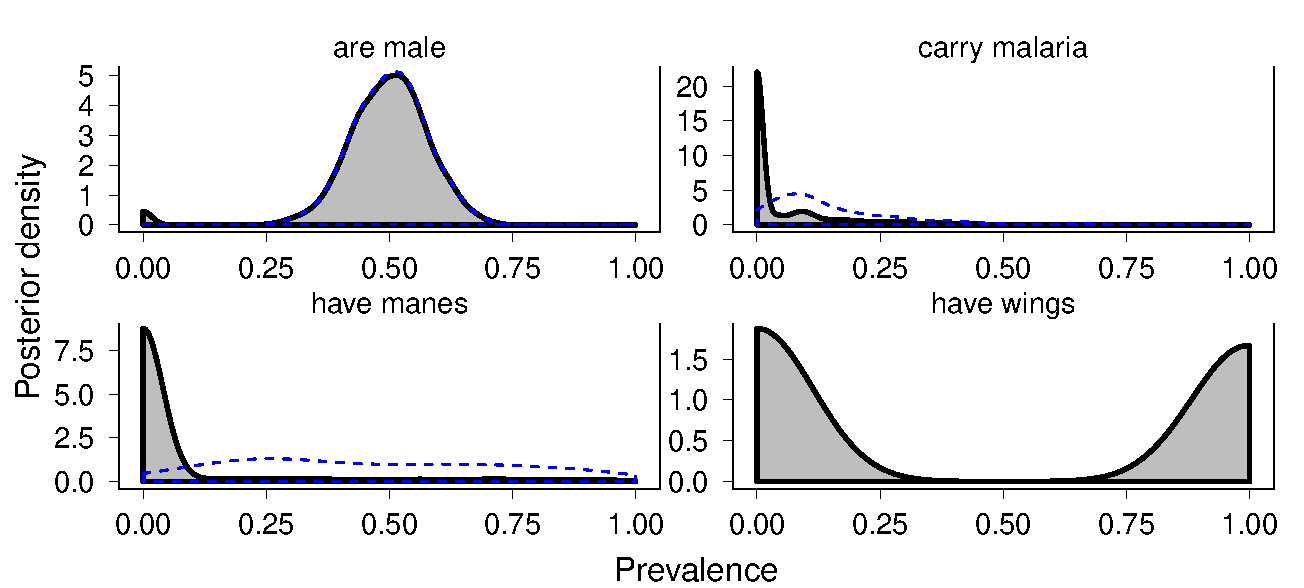
\includegraphics[width=0.8\columnwidth]{prevalence_priors_inferred-betas.pdf}
    \caption{Four example elicited prevalence priors. 
    Dotted lines show density by removing the mass at zero (corresponding to within-category prevalence). 
    For display purposes, this is omitted for ``have wings'', for which the density is off the scale and all at 1.
    Density plots reveal qualitatively different distributions for different properties. 
    Each sample from these distributions can be thought of to correspond to a particular animal category, representing the prevalence of the property within that animal category.
    Note the scale of the y-axis differs for each panel.}
  \label{fig:priors1a}
\end{figure}

There are substantial differences among the priors over prevalence between different types of properties. 
The distribution of ``has manes'' has the feature of being relatively rare across categories (large density at 0), and within a category there is considerable uncertainty in judgments as to what percentage of an arbitrary animal kind are expected have manes, though the expected value is around 50\% (Figure \ref{fig:priors1a} bottom left; within-category prevalence given by blue dotted line). 
By contrast, the distribution over ``is male'' has a lot less uncertainty: the property is highly prevalent across categories (almost no mass at 0), and within a category it is present in about 50\% of cases.
The property ``has wings'' is not particularly rare across categories (probably owing to the fact that bird categories are heavily represented in our stimulus set), and within a category is widespread, as reflected by the bimodal distribution. 
Finally, ``has malaria'' is an example of a property that is both rare across-species and within-species. 
The property is absent from most animal species, and even when it is present, it is only present in a small number of cases.

From this data, we can also estimate participants' beliefs about the prevalence of a property for a given category (e.g. the percentage of lions that have manes). The Maximum A-Posteriori (MAP) estimates and 95\% Bayesian Highest Density Intervals (HDI) over the mean prevalence for each property--category pairing of interest can be seen in Table \ref{tab:expt1}. 

With $P(x)$ empirically measured, the probabilistic model is fully specified. 
We compare the predictions of Eq.~\ref{eq:S2} to human judgments ($n=100$) about the acceptability of thirty generic sentences. 
We chose the sentences to cover a range of conceptual distinctions outlined by \citeA{Prasada2013}, including characteristic (e.g. ``Ducks have wings.''), minority (e.g. ``Lions have manes.''), striking (e.g. ``Mosquitos carry malaria.''), false generalization (e.g. ``Lions are male.''), and false (e.g. ``Lions lay eggs.'') bare plurals.

The 30 generic sentences fell into 3 \emph{a priori} categories: definitely true, definitely false, and neither true nor false (Figure \ref{fig:modeldataBars}, light bars). 
This \emph{a priori} distinction was a significant predictor of the eventual truth judgments: true generics were significantly more likely to be agreed with than the indeterminate generics ($\beta = 3.14; SE = 0.15; z = -20.9$), as revealed by a mixed-effect logistic regression with random by-participant effects of intercept.
Indeterminate generics were agreed with \emph{less} likely than chance ($\beta = -0.49; SE = 0.09; z = -5.3$) but significantly more than false generics ($\beta = 2.07; SE = 0.15; z = 14.1$).

About half of the variance in truth judgments are explained the prevalence of the property for the target category alone ($r^2 = 0.527$). 
This is, of course, expected given the existence of high-prevalence true generics (e.g. ``Leopards have spots.'') and low-prevalence false generics (e.g. ``Leopards have wings.''). 
However, large deviations from a purely within-category prevalence account remain: Generics with intermediate prevalences (prevalence quartiles 2 and 3: $ 22\% < prevalence < 62\%$), were not explained at all by prevalence ($r_{Q2,3}^2 = 0.006$).

\begin{figure}
\centering
    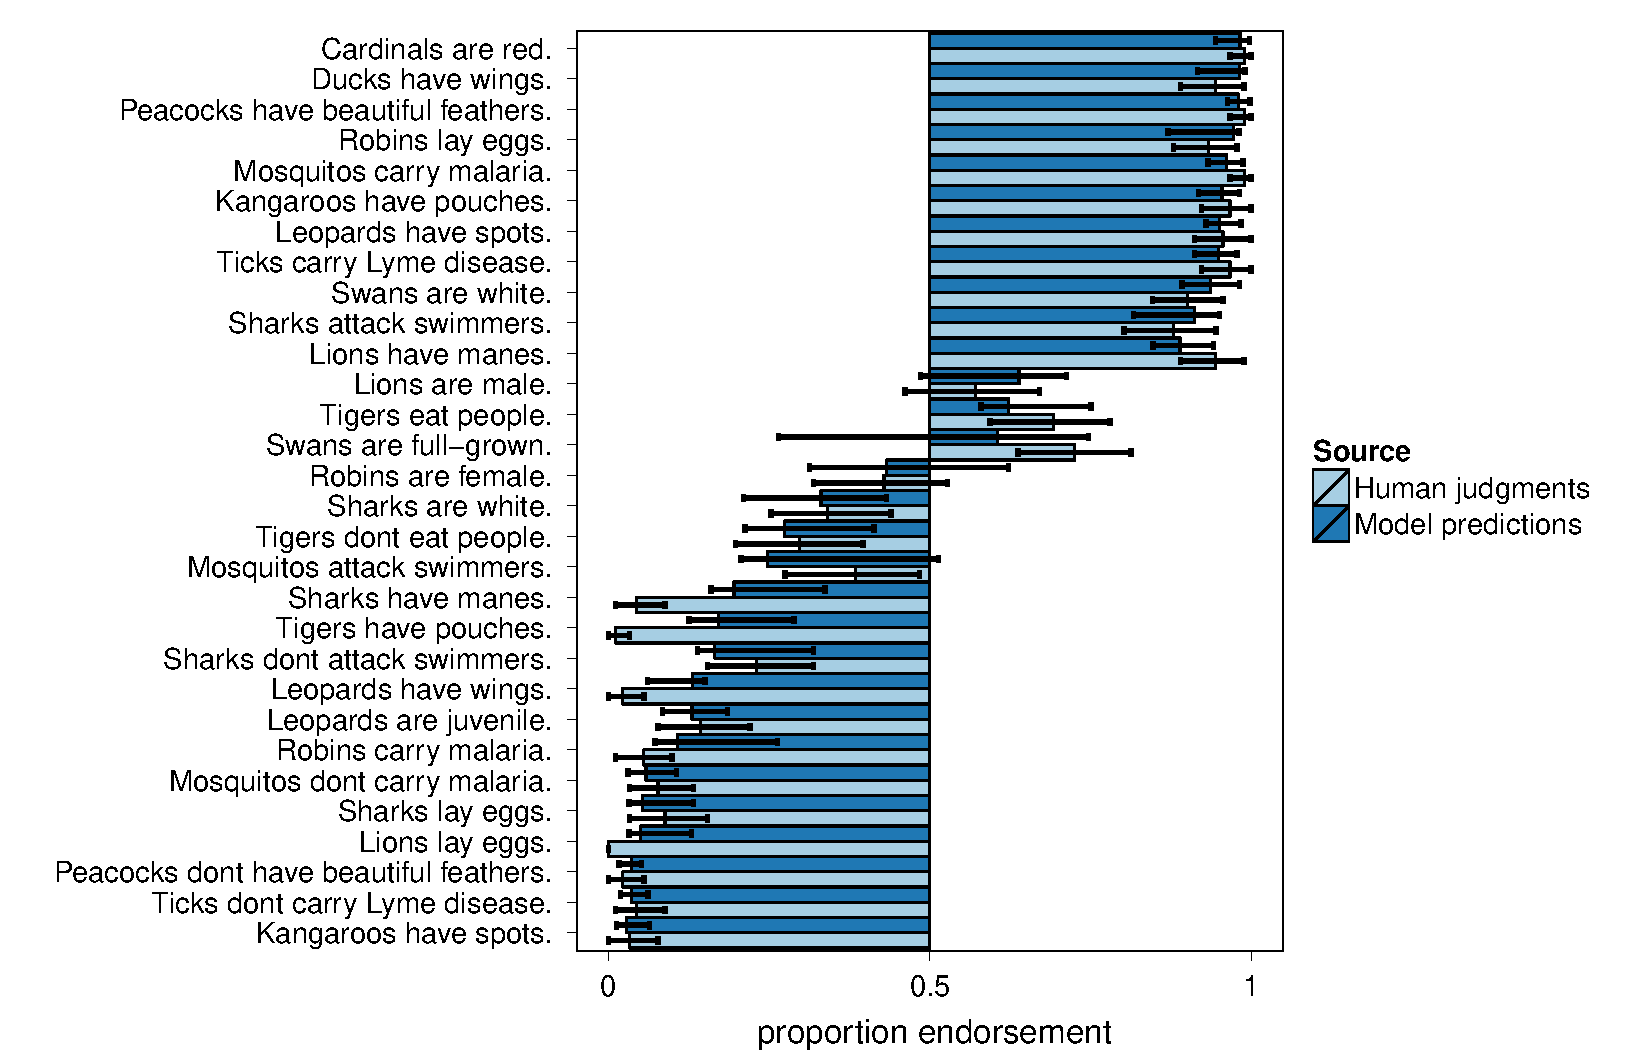
\includegraphics[width=\columnwidth]{tj_n100-postPred-byItem.pdf}
    \caption{Truth judgments from for thirty generic utterances and the predictive distribution for the lifted-variable model using empirical elicited priors. Order of the Y-axis corresponds to the rank-ordered model predictions. Error bars correspond with 95\% bootstrapped confidence intervals for the participant data and 95\% highest probability intervals for the model predictions.}
  \label{fig:modeldataBars}
\end{figure}

%\begin{figure}
%\centering
%    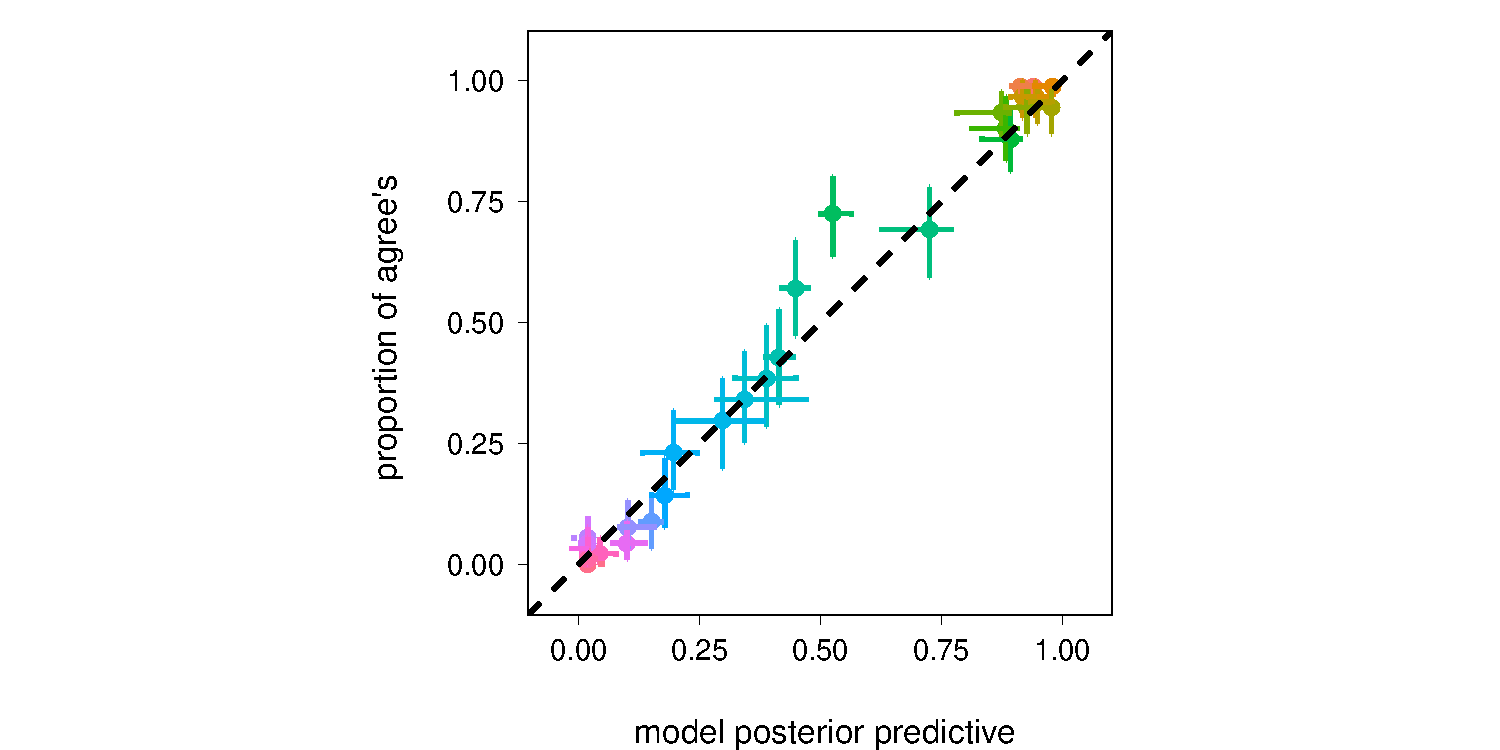
\includegraphics[width=\columnwidth]{tj_n100_tjVsPostpred_95hdi.pdf}
%    \caption{Truth judgments from Expt.~1b for each item vs. the posterior predictive MAP estimates for the target item using the lifted-threshold model with the empirical priors elicited in Expt.~1a. Color spectrum corresponds to the rank ordering of the truth judgment data; similarly colored dots received similar truth judgments. Error bars correspond with 95\% bootstrapped confidence intervals for the participant data and 95\% highest probability intervals for the model predictions.}
%  \label{fig:modeldataScatter}
%\end{figure}

The probabilisitic pragmatics model does a much better job of explaining the truth judgments ($r^2=0.974$). 
Generics that received definitive agreement or disagreement are predicted to be judged as such by the model (top and bottom portions of Figure \ref{fig:modeldataBars}). Unlike the model based on within-category prevalence alone, the lifted-threshold model does not break down for generics of categories with intermediate prevalence of the property (for prevalence quartiles 2 and 3, $r_{Q2,3}^2=0.975$. 

\subsubsection{Generics have strong implications (2500 words to this point)} 

Generic language exhibits mysterious behavior not only in how it is produced but in how it is understood.
Generics ``once accepted psychologically, ... appear to be commonly taken in a rather strong sense, as if the qualifier \emph{always} had implicitly crept into their interpretation'' \cite{Abelson1966}. \red{[Note: this is the same quote that Cimpian2010 use... is this okay?}.
%
\citeA{Gelman2002} found that adults interpret novel generic statements about familiar kinds (e.g. ``Bears like to eat ants.'') as implying that almost all of the category have the property (e.g. almost all bears like to eat ants).
%\citeA{Cimpian2010} found similar inferences with generics about unfamiliar kinds (e.g. ``Lorches have purple feathers.''). 

Interpretations of generic language are readily explored in our model of a listener (Eq.~\ref{eq:L1}) who hears a generic and is trying to infer what the world is like. 
Again, $P(x)$ was measured empirically.
Here, following \citeA{Cimpian2010}, we use novel animal categories and properties (e.g. ``Lorches'' and ``has purple feathers'') to explore how beliefs are updated by generic language. 
It is strange to measure participants' beliefs about these novel category---property pairs directly (e.g. answering ``How many lorches have purple feathers?'', without knowing what a lorch is).
Instead, we took advantage of the latent structure in the prior elicitation task (Expt.~1a) to ask participants ($n=40$) about the prevalence of a property (e.g. ``has purple feathers'') across-categories (e.g. ``How likely is it that \emph{there is a} lorch that has purple feathers?'') and within-categories (e.g. ``Suppose there is a lorch with purple feathers. What percentage of lorches do you think have purple feathers?''), separately. 
We used a hierarchical Bayesian approach to reconstruct the prevalence priors of a similar form to Expt.~1a (see Section \ref{sec:bda2} for details).

Classic work in generalization suggests that these prevalence distributions are different for different types of properties, including different types of conceivably biological properties \cite{Nisbett1983}. 
We used 4 different types of properties: body parts (e.g. ``has claws'') , colored body parts (e.g. ``has purple feathers''), biological adjectives (e.g. ``has small wings''), and common accidental or disease states (e.g. ``has wet fur'') and rare accidental or disease states (e.g. ``has broken legs'')\footnote{The distinction between common and rare accidental properties was determined empirically by oversampling those properties, analyzing the data first by item, and performing a median split based on the \emph{a priori} believed prevalence of the property}.

Figure \ref{fig:prior2} (left) shows the inferred distributions for prevalence $x$ for 5 different types of properties. 
Figure \ref{fig:prior2} (right) shows the region of interest of these distributions by removing the mass at 0. 
With the exception of the body part category, properties are mostly likely to be absent from the category (Figure \ref{fig:prior2} left; modes of distributions are at 0).
If the property is present in the category, the most likely prevalence for biological properties (``part'', ``color part'', and ``vague part'') is 100\% (Figure \ref{fig:prior2} right; modes of blue, green, and red distributions are at 1).
This is not the case with the prevalence priors for accidental properties, for which lower values are more likely (Figure \ref{fig:prior2} right; modes of orange and purples distributions are at some low prevalence).


\begin{figure}
\centering
    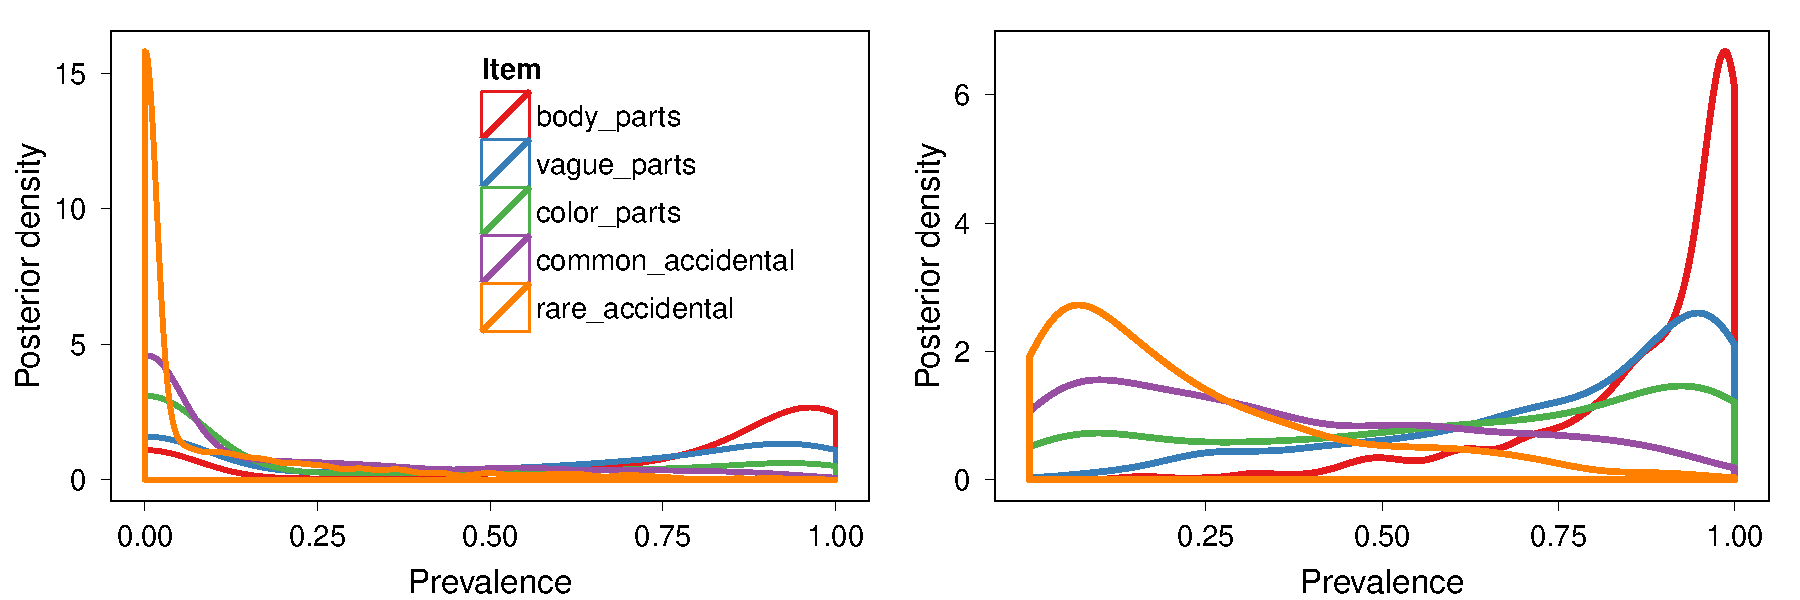
\includegraphics[width=\columnwidth]{prior2_prevalenceprior-50k.pdf}
    \caption{Prevalence priors inferred from the prior elicitation experiment  (Expt.~1a). Right plot shows all non-zero probability mass. This corresponds to the expected within-category prevalence. Different types of properties have different likely prevalence values.}
  \label{fig:prior2}
\end{figure}

We compared the interpretations of the pragmatic listener in Eq.~\ref{eq:L1} to the participants judgments ($n=40$) about the likely prevalence of the property after hearing a generic (e.g. ``Lorches have purple feathers.''), in the same spirit as \citeA{Gelman2002}. Also following \citeA{Cimpian2010}, we recruited participants ($n=40$) to help determine the average prevalence at which a speaker would assent to the generic, which was previously found to be not as sensitive to participants beliefs about the property (but, cf. \citeA{Cimpian2010}, Expt.~4).

Implied prevalence of the generic was affected by the type of property in question (Figure \ref{fig:exp2b} Left; dark bars). 
%Of theoretical interest is whether or not the median split we performed on the accidental properties based on the results of the prior elicitation experiment resulted in different implications for the associated generic.
Interestingly, we observe greater implied prevalence of common accidental properties than rare accidental properties, given our median split based on the prior elicitation task ($\beta=0.061; SE = 0.025; t(39) = 2.47; p = 0.018$) \footnote{These statistics are the result of a mixed-effects linear regression with a maximal mixed-effect structure: Random by-participant effects of intercept and slope}.
Implications of generics of body parts was significantly greater than those of the biological properties used by \citeA{Cimpian2010} (here, ``color parts'') ($\beta=0.118; SE = 0.024; t(39) = 4.74; p < 0.001$).
There was also a trending effect for the implications of vague body parts (e.g. curly fur) to be greater than those of color parts (e.g. yellow fur) ($\beta=0.032; SE = 0.016, t(54.8) = 1.95; p = 0.056$), possibly due to the belief that the same kind of animal can come in many different colors (e.g. dogs).
Also consistent with previous findings, there were no differences in the tendency to agree with the generic based on property type (Figure \ref{fig:exp2b} left; light bars)

\begin{figure}
\centering
    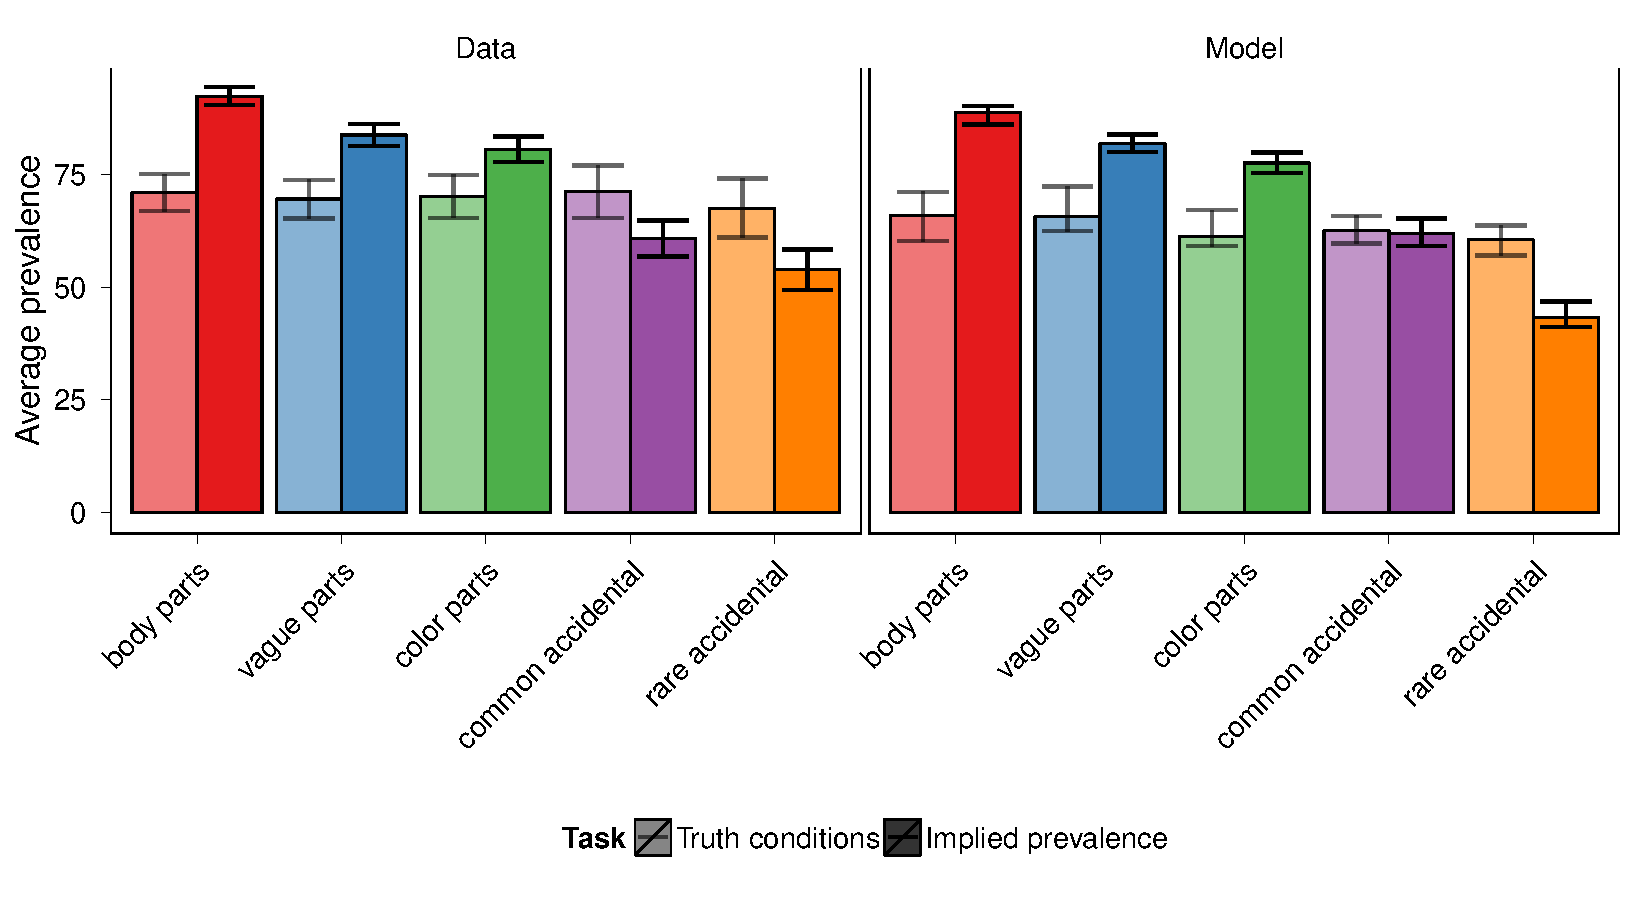
\includegraphics[width=\columnwidth]{asym-data-model-2phi-2so-50k.pdf}
    \caption{Generic utterances of unfamiliar categories truth conditions and implied prevalence (left) and model predictions (right). 
    This replicates and extends Cimpian et al. (2010). 
    Generic statements are accepted for a range of prevalences, resulting in an intermediate average prevalence (light bars) for ``truth conditions''. 
    Upon hearing a generic statement about biological properties, participants' infer that a high proportion of the category has the property (dark bars: red, blue and green). 
    Generics about accidental properties do not result in such a high implied prevalence (dark bars: purple and orange).  
    Error bars denote bootstrapped 95\% confidence intervals for the data and Bayesian 95\% credible intervals for the model.}
  \label{fig:exp2b}
\end{figure}


We compared this behavioral data to our model by using the speaker model (Eq.~\ref{eq:S2}) to predict the truth judgments task (as in Expt.~1) and using the listener model (Eq.~\ref{eq:L1}) to predict the interpretation task. 
We submitted our speaker model to the same analysis as the truth judgments data, following \citeA{Cimpian2010} (see Supplement). 
The speaker model did not make different predictions as to the average acceptability prevalence to produce the generic (Figure \ref{fig:exp2b}, Right, light bars). 
At the same time, the listener model produced variable interpretations contingent on the type of property under discussion (Figure \ref{fig:exp2b}, Right, dark bars). These inferences align almost perfectly with participants productions and interpretations of novel generic utterances ($r^2(10) = 0.93$). 

How does the model capture these fine-grained inferences that listeners draw?
Consider again the belief distributions about the properties inferred from Expt.~2a (Figure \ref{fig:prior2}). 
All of the properties have substantial mass at 0 (Figure \ref{fig:prior2} Left). 
This gives the speaker validity in saying the generic at low prevalence levels (though the speaker's confidence in doing so increases as prevalence increases).
The listener has the complementary task: She brings \emph{a priori} uncertainty about the generic threshold to the table.
Consider what would happen if she inferred the most conservative threshold (0) and responded with the \emph{maximum a posteriori} (MAP) of the distribution. 
A threshold of 0 produces Figure \ref{fig:prior2} (right), because it only rules out the possibility that 0\% of the category has the property. 
The resulting peaks (MAPs) of the distributions are near 1 for biological properties (parts, color parts, vague parts) and around 10\% for accidental properties (both rare and common). This alone would produce variable interpretations. 
Our listener, however, does something wiser: She integrates over her uncertainty about the threshold (believing the speaker to be not just truthful but informative as well), and produces interpretations that both take reflect the whole distribution.
This results in subtle differences between the implications of body parts (e.g. ``Lorches have wings.'') and  color parts (e.g.``Lorches have purple wings.''), and differences in interpretations of rare and common accidental properties. 


\subsubsection{Conclusions (4000 words up to now)}

It might seem paradoxical that a part of language that gets so much usage should be vague. 
Shouldn't speakers want to express their ideas as clearly as possible?
Language evolutionary pressures suggest that, to the contrary, such underspecification is in fact useful, given that there is some context through which the uncertainty can be resolved \cite{Piantadosi2012}.
In this work, context takes the shape of a listener and speaker's shared beliefs (i.e. common ground) about the property in question. 
This, coupled with standard inferences from conversational pragmatics, allows the listener to figure out the meaning of the otherwise underspecified utterance.

Interpretation of generic language is strongly governed by listeners' beliefs about the domain in question. 
The generic, it would seem, doesn't convey any additional information beyond what the listener already knew about the domain.
This shouldn't surprise us. 
In much the same way, ``John is tall'' does not actually tell a listener about what \emph{tall} means\footnote{However, ``John is a person'' does tell a listener about what \emph{tall} means in ``John is tall''.}. 
Rather, the listener is expected to come to the conversation with some beliefs about heights, and knowing that John is a person, be able to infer likely meanings for \emph{tall}.

Where might these shared beliefs come from?
It is quite plausible that these distributions are derived from higher-order conceptual knowledge about the nature of these properties \cite{Gelman2005, Keil1992}.
Much of the psychological and philosophical work has looked beyond prevalence and focused on conceptual distinctions among generics \cite{Prasada2013, Leslie2008}. For example, \citeauthor{Prasada2013} has argued for a distinction between \emph{characteristic} properties (e.g. ``Diapers are absorbent.'') and \emph{statistical} properties (e.g. ``Diapers are white.'').
 Where in the prevalence-based semantics could such conceptual distinctions come into play?
Probabilistic models are a useful way to represent rich, structured knowledge of world \cite{Goodmanconcepts}. It's plausible that the prevalence distributions focused on in this work are derived from richer conceptual knowledge. For the purpose of the semantics of generics, prevalence is sufficient to capture the range of truth judgments  and interpretations for these sentences. How interlocutors arrive at estimates of the prevalence, or the prevalence distribution at large, may be the result of a probabilistic, conceptual model of the world. 

This formalism gives a new, computational perspective on how ideas are conveyed and how beliefs play a central role in understanding language.
Generics are vague, but predictable and useful.


\bibliographystyle{apacite}

\setlength{\bibleftmargin}{.125in}
\setlength{\bibindent}{-\bibleftmargin}

\bibliography{generics}


\end{document}
